
\chapter{Jet Classification at the LHC}
\label{ch:tagging}

Jet classification, commonly referred to as ``jet tagging'', was one of the first applications of deep learning in particle physics and remains arguably the most important.
The techniques covered in this chapter are used by both ATLAS and CMS and are driving improvements in the search for di-Higgs production, which is the main goal of the current LHC physics program.
This chapter will introduce jet tagging as a problem, then cover an ATLAS study on top tagging that is the first original research contribution in this thesis.
It will close with a discussion of how jet tagging has progressed since the publication of the ATLAS top tagging paper and end with some prospects for the high luminosity LHC.

\section{Jet Tagging}
\label{sec:tagging-intro}

Most searches and measurements at the LHC are concerned with the high-energy scattering of partons.
Ideally one would directly measure the identity and kinematics of the individual quarks and gluons produced in an LHC collision.
In practice, the parton shower and hadronization processes make this impossible.
Detectors can only observe the outcome of the parton shower and hadronization processes, which are collimated sprays of hadrons known as jets.
See \Cref{ch:qcd} for a full discussion.
These jets are typically used as proxies for the initiating parton.
For example the kinematics of the initiating parton can be inferred from the kinematics of the jet, obtained by summing the four-momenta of the jet's constituent hadrons.
Inferring the \emph{type} of parton that initiated the jet is the problem of jet tagging.

\begin{figure}[tb]
    \centering
    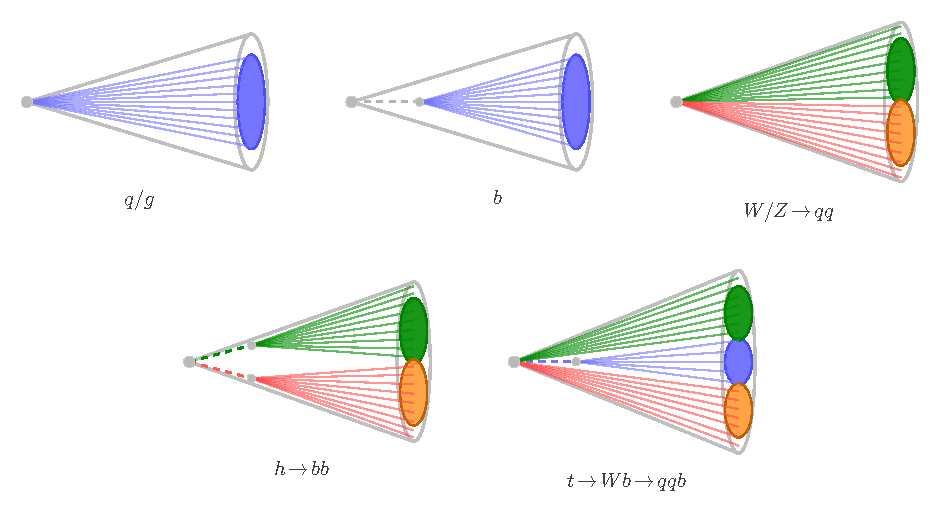
\includegraphics[width=0.85\linewidth]{figures/ch4/jet_types_diagram.pdf}
    \caption{Schematic illustration of the two broad categories of jets produced in LHC collisions. From the top left working clockwise: light quark and gluon initiated jets are the most abundant jets with no substructure, bottom quark (and to some extent charm quark) initiated jets conain a displaced vertex due to the long-lived B and D hadrons, jets initiated by the hadronic decay of the W and Z bosons contain a two-pronged substructure, jets initiated by the decay of a Higgs boson to two b quarks results in a two-pronged substructure with displaced vertices, and the hadronic decay of a top quark results in a three-pronged substructure with one displaced vertex.}
    \label{fig:jet-types}
\end{figure}

Historically, two distinct jet tagging problems have been studied at the LHC.
The first is \textit{boosted jet tagging}.
When a massive particle such as a top quark, $W$ or $Z$ boson, or Higgs boson is produced with a transverse momentum much larger than its mass ($p_T \gg m$), its hadronic decay products are emitted nearly collinearly.
The resulting jets from each daughter quark merge into a single large-radius jet with non-trivial substructure.
$W/Z/H \to q\bar{q}$ decays produce a two-pronged substructure, and a $t \to Wbq\bar{q}$ decay produces a three-pronged substructure.
Identifying these boosted jets against the large background of high-\pt light-quark and gluon jets requires exploiting this substructure.
Early methods for doing so relied on multivariate discriminants such as BDTs or shallow neural networks trained on a set of hand-engineered substructure observables~\cite{Altheimer:2013yza, Thaler:2008ju}.
An example use case for boosted jet tagging is to search for BSM resonances that decay to boosted SM objects like top quarks of W/Z bosons~\cite{ATLAS:2022enb,CMS:2026ogg}.

The second category is \textit{flavor tagging}.
When a bottom or charm quark is produced in the hard scatter, the resulting jet contains a $B$ or $D$ hadron.
These hadrons are long-lived relative to the light hadrons produced in light-quark and gluon jets, and they therefore travel a measurable distance before decaying, leaving a displaced secondary vertex inside the jet.
Identifying jets that contain $B$ or $D$ hadrons as opposed to jets from light quarks or gluons is called $b$- or $c$-tagging.
As in the boosted case, early flavor taggers reconstructed the displaced vertex explicitly and used this information as an input to a BDT or neural network~\cite{ATLAS:2016gsw}.

The types of jets are illustrated in \Cref{fig:jet-types}.
Boosted jet tagging aims to identify top, W/Z, and Higgs jets against the background of light-quark and gluon jets, and flavor tagging aims to identify $b$ and $c$ jets\footnote{Note that $c$ jets are not shown in the Figure but are a distinct category of jets from $b$ jets though they're signatures are very similar.}.
Both are classification tasks, where one must distinguish a signal jet from a background jet using the kinematics of the jet constituents that are measured by the detector.
The distinction is the nature of the discriminating information.
Boosted tagging relies on the global spatial structure of constituent particles within a jet, while flavor tagging relies on the longitudinal and transverse impact parameter information of the tracks within a jet that are used to reconstruct secondary vertices.
These sets of information are not independent, but do factorize somewhat into signals coming from the inner tracking and calorimeter sub-systems of the ATLAS and CMS detectors.

Both problems have a long history in collider experiments.
In runs one and two of the LHC, both were solved by combining hand-engineered expert features with a simple multivariant discriminant provided by a BDT or small neural network.
The story of the top tagging paper presented here is that larger neural networks that operate directly on the jet constituent kinematics rather than on hand-engineered features can achieve much better performance.
While this is illustrated in a boosted jet tagging task, the same is true for flavor tagging.

The paper focuses on boosted top tagging, a particular boosted jet tagging task that classifies top quark initiated jets against the light quark and gluon initiated (sometimes called QCD) background.
Boosted top tagging is the prototypical multi-prong jet tagging problem and was the subject of many early deep learning applications in particle physics.
The study presented here, carried out in 2022--2023, constitutes the first original research contribution of this thesis.
The lessons drawn from the binary top-versus-QCD classification problem remain relevant to large multi-class taggers of today, to which I will return in \Cref{sec:tagging-future}.

\section{Constituent Based Top Quark Tagging}
\label{sec:constituent-top-tagging}

\subsection{The Top Tagging Landscape}

Before describing the ATLAS study, it is useful to place it in context.
In 2019, a community comparison study~\cite{Kasieczka:2019dbj} trained a wide variety of deep learning based top tagging methods on a single, common dataset and evaluated their performance under identical conditions.
The study serves as the clearest demonstration of the state of constituent-based top tagging prior to the ATLAS work described here.
The key result is summarized by the ROC curve reproduced in \Cref{fig:landscape-roc}.

\begin{figure}[tb]
    \centering
    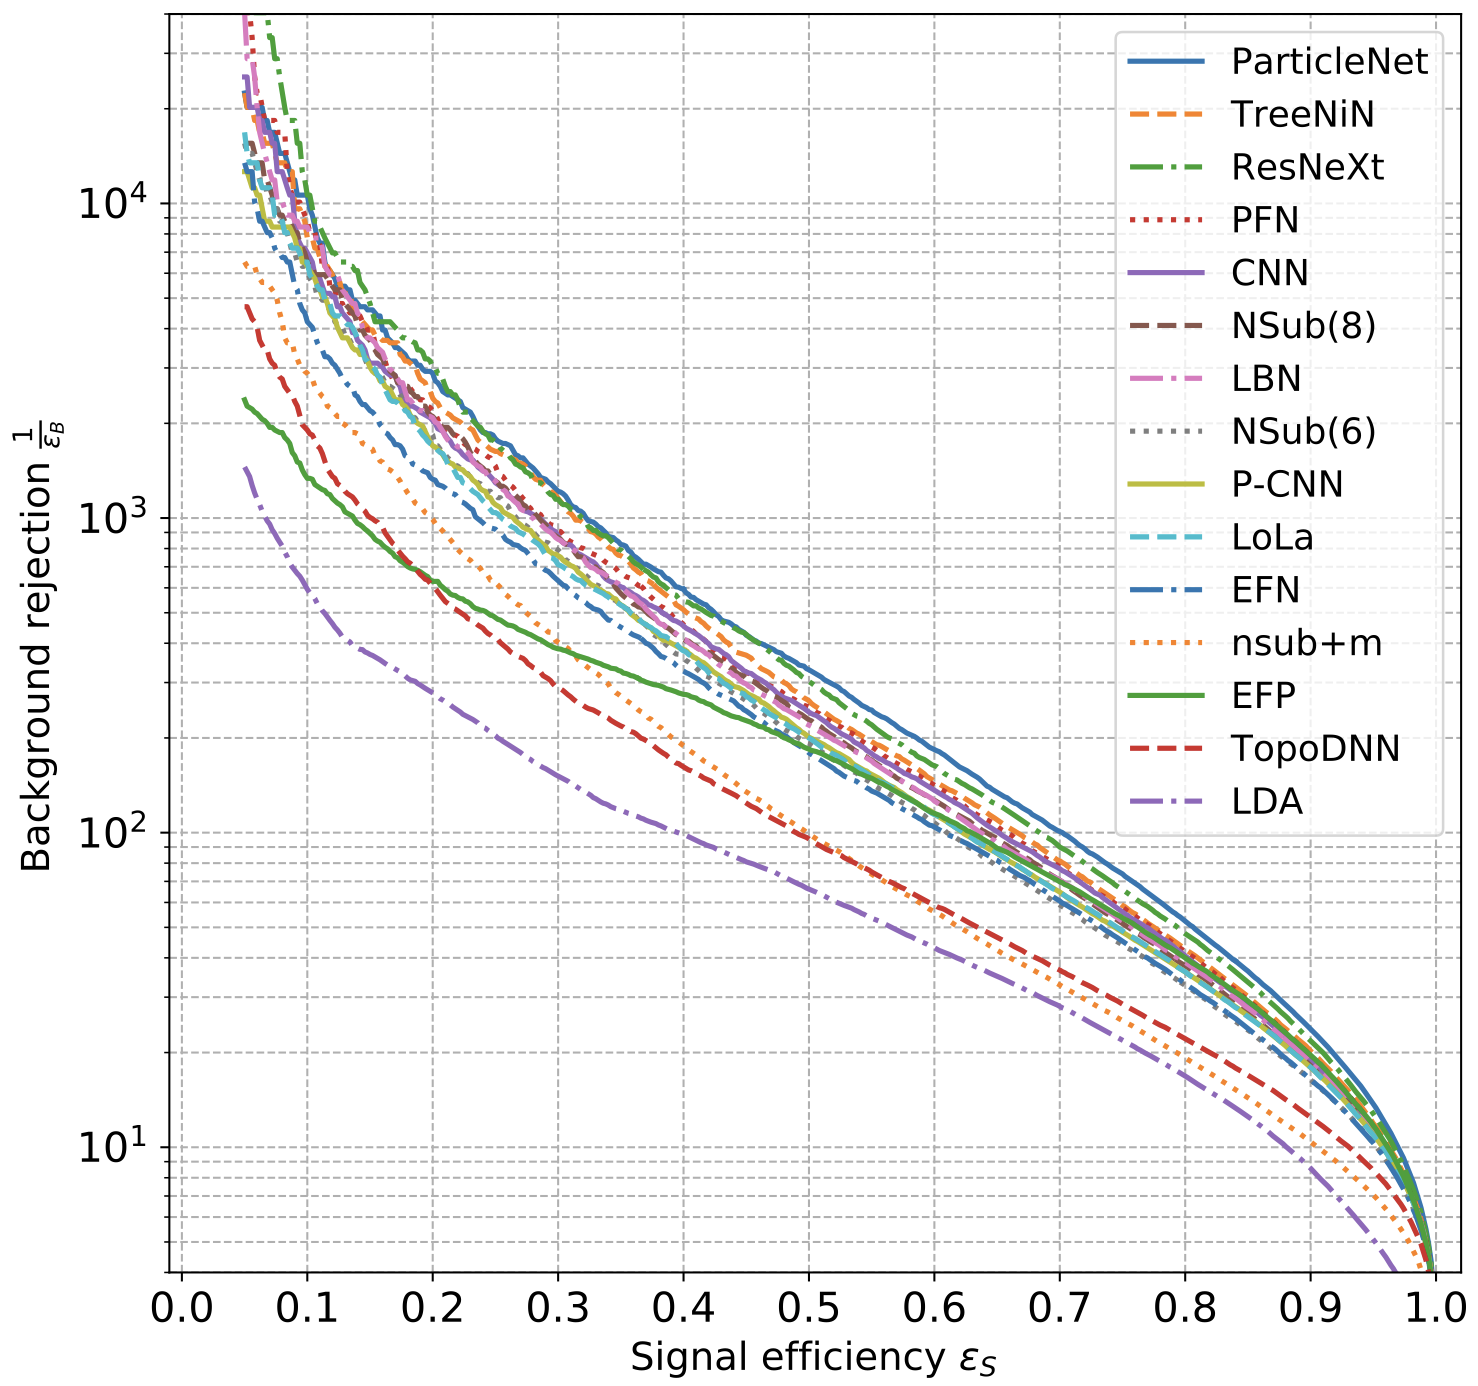
\includegraphics[width=0.8\linewidth]{figures/ch4/landscape_roc.png}
    \caption{ROC curves for a range of top tagging classifiers evaluated on a common dataset, reproduced from Ref.~\cite{Kasieczka:2019dbj} under the Creative Commons Attribution 4.0 International license. Each curve traces the signal efficiency (true positive rate) against the background rejection (inverse false positive rate) as the classifier threshold is varied. A classifier with no discriminating power would follow the diagonal; greater area under the curve indicates better classification performance. Constituent-based deep learning taggers (upper left cluster) consistently outperform the expert-feature baseline (lower left).}
    \label{fig:landscape-roc}
\end{figure}

A ROC (receiver operating characteristic) curve plots signal efficiency on the horizontal axis against background rejection on the vertical axis, as the discriminant threshold of the classifier is swept from its most to least restrictive value.
A tagger with no discriminating power produces a flat line (all thresholds yield the same background rejection regardless of signal efficiency), while a perfect tagger reaches the upper-left corner of the plane.
The area under the curve (AUC) summarizes overall classification power in a single number, with a perfect classifier achieving an AUC of 1.

The landscape study yields two important takeaways.
First, constituent-based deep learning taggers substantially outperform methods that rely on hand-engineered expert features.
This is the jet tagging analog of the AlexNet moment: rather than asking domain experts to distill the relevant physics into a set of high-level variables, end-to-end networks learn directly from the raw kinematic information of the jet constituents which patterns discriminate top jets from QCD.
The improvement in background rejection is a factor of several relative to the expert-feature baseline.
Second, the dataset used in the landscape study was generated with the fast detector simulation Delphes~\cite{deFavereau:2013fsa}, which models the detector response at a coarse level.
The much more realistic \textsc{Geant4}-based full simulation used by ATLAS and CMS introduces detector effects, such as calorimeter cell geometry and noise, that are absent from Delphes.
Whether the performance advantage of constituent-based taggers persists under realistic simulation was an open question.
Furthermore, the landscape study evaluated only raw classification power.
Deploying taggers in physics analyses requires a careful treatment of systematic uncertainties, which was entirely absent from the landscape comparison.

\subsection{Dataset and Jet Selection}

The primary objective of Refs.~\cite{ATLAS:2022qby, ATLAS:2024rua} was to address both of these gaps: train and evaluate top taggers on ATLAS full simulation, and provide a high-quality public dataset to support future studies.

The first step is to construct a dataset of labeled jets from simulated events.
Simulation is necessary because truth labels are required for the supervised training of classifiers.
Top quark signal jets are obtained from simulated $Z' \rightarrow t\bar{t}$ events with $m_{Z'} = 2$~TeV, where the $Z'$ is a hypothetical massive resonance used solely as a convenient source of boosted top quarks.
The production cross section is reweighted to yield an approximately flat jet $p_T$ distribution, which ensures that the tagger performance is not driven by the particular kinematic configuration of the training sample.
Background jets are obtained from simulated QCD dijet events.

Jets are clustered from Unified Flow Object (UFO) inputs~\cite{ATLAS:2020gwe}.
The UFO is an ATLAS analysis object specifically optimized for reconstructing large-radius jets with significant substructure.
It combines inner detector tracking and calorimeter information in a way that exploits the complementary resolution of the two sub-systems.
The four-momenta of the UFO constituents within each jet are the inputs to the constituent-based taggers described below.

A jet selection is then applied to both samples.
\Cref{tab:cuts} summarizes the requirements.
Basic kinematic requirements are applied to all jets.
For the signal sample, additional truth-level requirements define the top quark jet label: the jet must be geometrically matched to both a truth jet and to the truth top parton, have a groomed mass consistent with the top quark mass, contain at least one ghost-associated $b$-hadron (ensuring the jet contains the $b$-quark from the top decay), and satisfy a requirement on the truth jet splitting scale $\sqrt{d_{23}}$ that ensures all three top decay products are captured within the jet.
The $\sqrt{d_{23}}$ requirement has an explicit $p_T$ dependence that accounts for the increasing collimation of the decay products at higher jet $p_T$.
After selection, the dataset consists of top quark jets (signal) and QCD jets (background), with the goal of training classifiers that separate them.

\renewcommand{\arraystretch}{1.5}
\begin{table}[]
    \centering
    \begin{tabular}{l|l}
        \hline
        \hline
        Jet Requirements & Top quark jet requirements \\ \hline 
        Jet  $|\eta| < 2.0$ & $dR(\text{jet, truth jet}) < 0.75$ \\
        Jet  $p_{\text{T},\text{truth}} > 350$ GeV & $dR(\text{truth jet, top parton}) < 0.75$ \\
        Number of constituents $\geq 3$ & Ungroomed truth jet mass $> 140$ GeV \\
        Jet mass $> 40$ GeV & Number ghost associated $b$-hadrons $\geq 1$ \\
         & Truth jet $\sqrt{d_{23}} > \exp (3.3 - \num{6.98e-4} \times \text{truth jet} \: \pT)$ \\ \hline \hline
    \end{tabular}
    \caption{A summary of the requirements applied on all of the jets in the simulation samples to produce the training and testing sets. The additional top quark jet requirements constitute the truth labeling strategy, and are only applied to jets in the sample of simulated top quarks.}
    \label{tab:cuts}
\end{table}


\subsection{Tagger Architectures}

Five classifiers spanning a range of architectural complexity are trained and evaluated.
The architectural building blocks have been introduced in \Cref{ch:ml}; only the jet-tagging-specific details are described here.

\textbf{hlDNN.} A multi-layer perceptron trained on 15 hand-engineered substructure variables.
This serves as the expert-feature baseline for the study.

\textbf{DNN.} A multi-layer perceptron that operates directly on the constituent four-momenta, with no hand-engineered features.
Because the number of constituents varies from jet to jet, the constituent list is zero-padded to a fixed length before being passed to the network.

\textbf{EFN and PFN.} The Energy Flow Network and Particle Flow Network are deep set architectures~\cite{Komiske:2018cqr}.
Each constituent is mapped independently through a shared per-constituent network to produce a latent representation; the representations are then aggregated (summed) to produce a jet-level embedding, which is passed to a final classifier network.
The EFN is constrained to be infrared and collinear (IRC) safe: constituent coordinates are weighted by their $p_T$ fraction before aggregation, so the network output is invariant under the addition of soft particles or the collinear splitting of any constituent.
This constraint limits the information available to the EFN but, as will be discussed in the following section, confers significant robustness against systematic uncertainties.

\textbf{ResNet50.} A convolutional neural network~\cite{He:2015resnet} applied to jet images.
A jet image is constructed by projecting the constituent $p_T$ onto a $64 \times 64$ pixel grid in the $(\eta, \phi)$ plane centered on the jet axis, with each pixel value equal to the sum of constituent $p_T$ falling within it.
Pixel intensities are rescaled as $p_T \to \log(1 + 100\, p_T)$ to enhance sensitivity to the lower-$p_T$ substructure patterns that would otherwise be washed out by the hardest constituents.
Example jet images are shown in \Cref{fig:jet-images}.
The three-pronged substructure of the top jet is visible as an over-density of radiation at three locations around the jet center in the ratio image.

\begin{figure}[tb]
    \centering
    \begin{subfigure}[b]{0.32\textwidth}
        \centering
        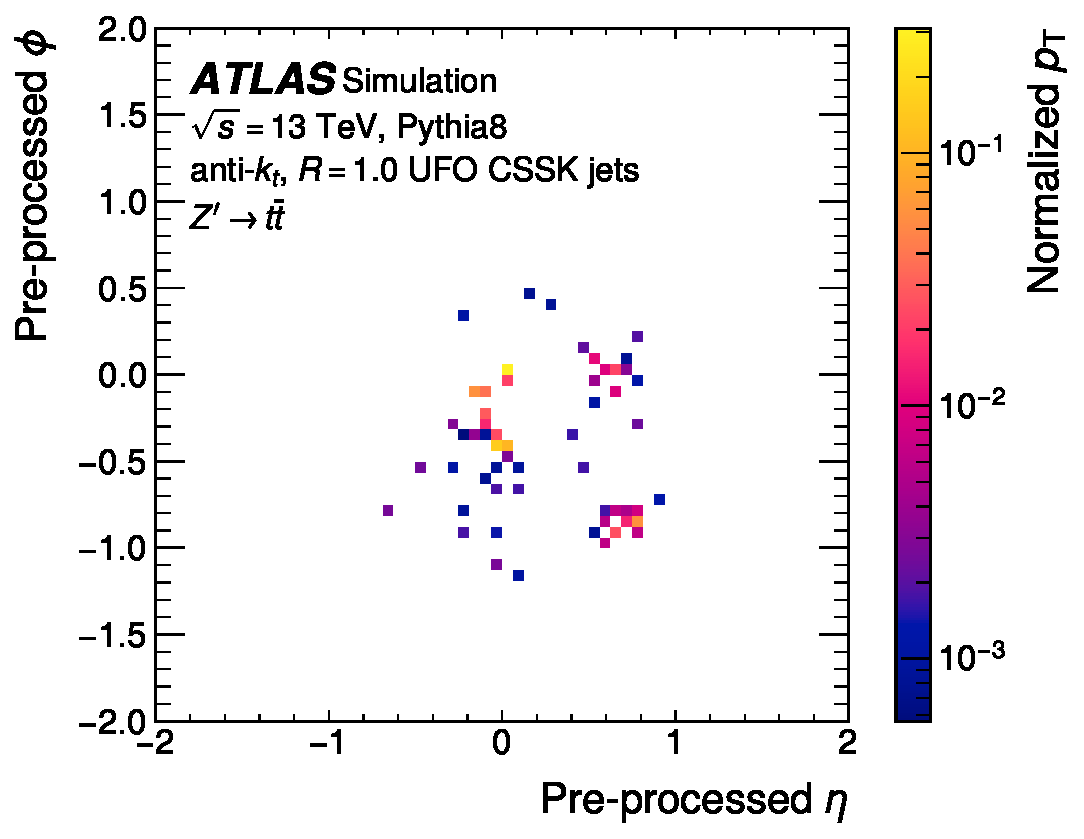
\includegraphics[width=\linewidth]{figures/ch4/top_jet.pdf}
        \caption{Average top jet image.}
        \label{fig:top-jet-image}
    \end{subfigure}
    \hfill
    \begin{subfigure}[b]{0.32\textwidth}
        \centering
        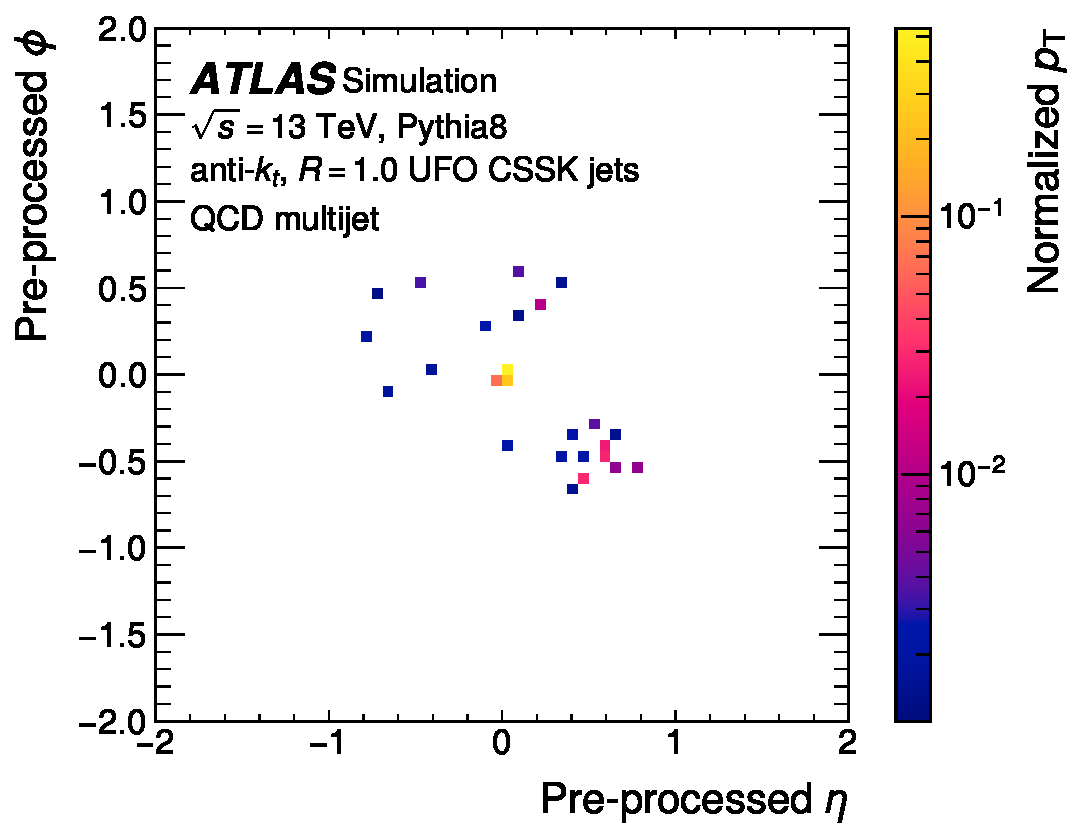
\includegraphics[width=\linewidth]{figures/ch4/qcd_jet.pdf}
        \caption{Average QCD jet image.}
        \label{fig:qcd-jet-image}
    \end{subfigure}
    \hfill
    \begin{subfigure}[b]{0.32\textwidth}
        \centering
        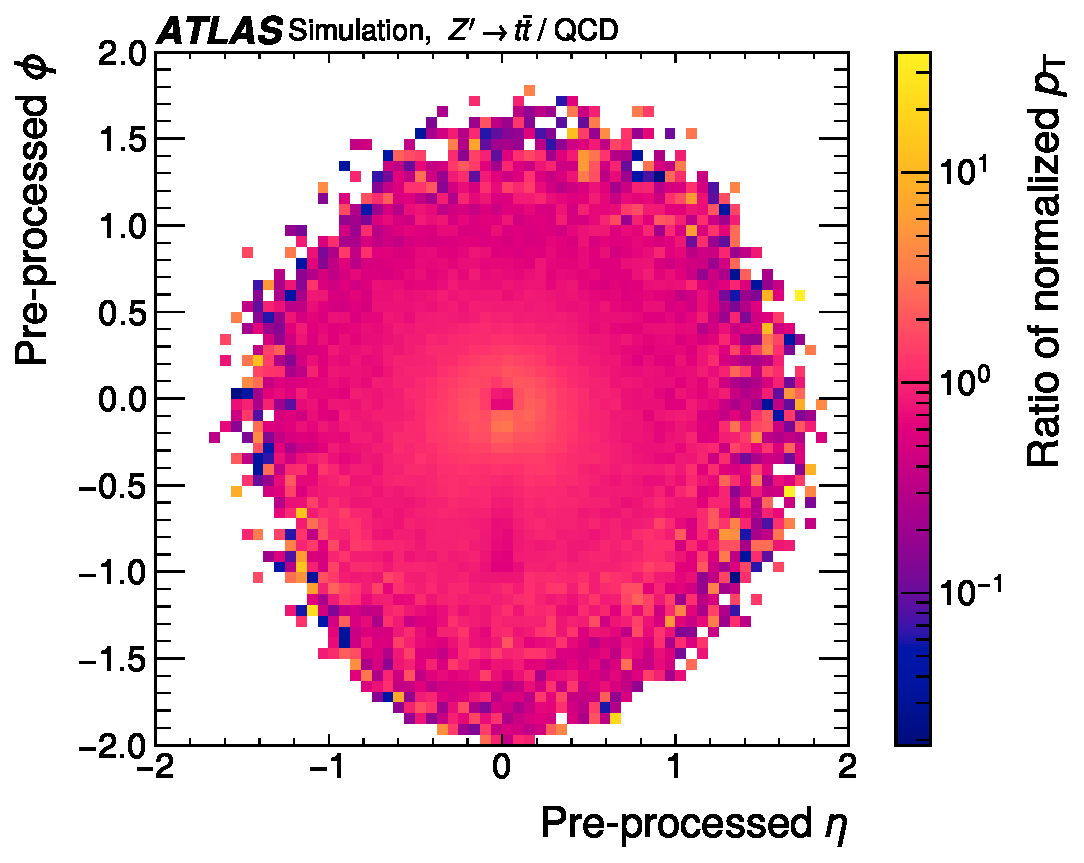
\includegraphics[width=\linewidth]{figures/ch4/jet_image_ratio.pdf}
        \caption{Ratio: top / QCD.}
        \label{fig:jet-image-ratio}
    \end{subfigure}
    \caption{Average jet images for top quark jets (left) and QCD jets (center), and their pixel-wise ratio (right). Pixel intensities are shown on a logarithmic scale after the $p_T \to \log(1 + 100\,p_T)$ rescaling. The three-pronged substructure of the top quark decay is visible as the three over-dense regions surrounding the jet center in the ratio image.}
    \label{fig:jet-images}
\end{figure}

\textbf{ParticleNet.} A dynamic graph convolutional neural network~\cite{Qu:2019gqs}.
Each jet constituent is represented as a node, with node features given by the seven input variables described below.
In the first message-passing layer, edges connect each node to its $k = 18$ nearest neighbors in the $(\eta, \phi)$ plane, incorporating the inductive bias that spatially proximate constituents are physically related.
In subsequent layers, nearest neighbors are determined in the full feature space rather than the coordinate subspace, so the graph topology changes dynamically after each block.
ParticleNet has been deployed extensively by CMS for jet tagging in a wide range of measurements and searches, making it one of the most practically important architectures in LHC physics.

\subsection{Input Features and Training}

Each constituent-based tagger operates on a common set of seven input features per constituent: the $\eta$ and $\phi$ coordinates relative to the jet axis, the logarithms of the constituent $p_T$ and energy $E$, the logarithms of the constituent $p_T$ and $E$ normalized to the total jet $p_T$ and $E$ respectively, and the angular distance $\Delta R$ between the constituent and the jet axis.
The EFN uses only constituent $\eta$, $\phi$, and $p_T$ by architectural constraint, and the ResNet50 uses the jet image rather than per-constituent features.

All taggers are trained using the Adam optimizer to minimize the binary cross-entropy loss.
Training proceeds until the validation loss fails to improve for 20 consecutive epochs.
The training, validation, and test sets contain 9 million, 1 million, and 3.8 million jets respectively.

\subsection{Results}

The classification performance of each tagger is summarized in \Cref{tab:performance_numbers} and \Cref{fig:roc}.
Three metrics are reported: the AUC, the accuracy (ACC), and the inverse background rejection $\varepsilon^{-1}_\text{bkg}$ evaluated at fixed signal efficiencies of 50\% and 80\%.
The inverse background rejection is the most physically relevant metric for collider analyses: downstream measurements and searches typically operate at a fixed working point (a fixed signal efficiency), and the figure of merit is how many background jets survive the cut, since fewer background events in the signal region directly translates to improved sensitivity.

\begin{figure}[tb]
    \centering
    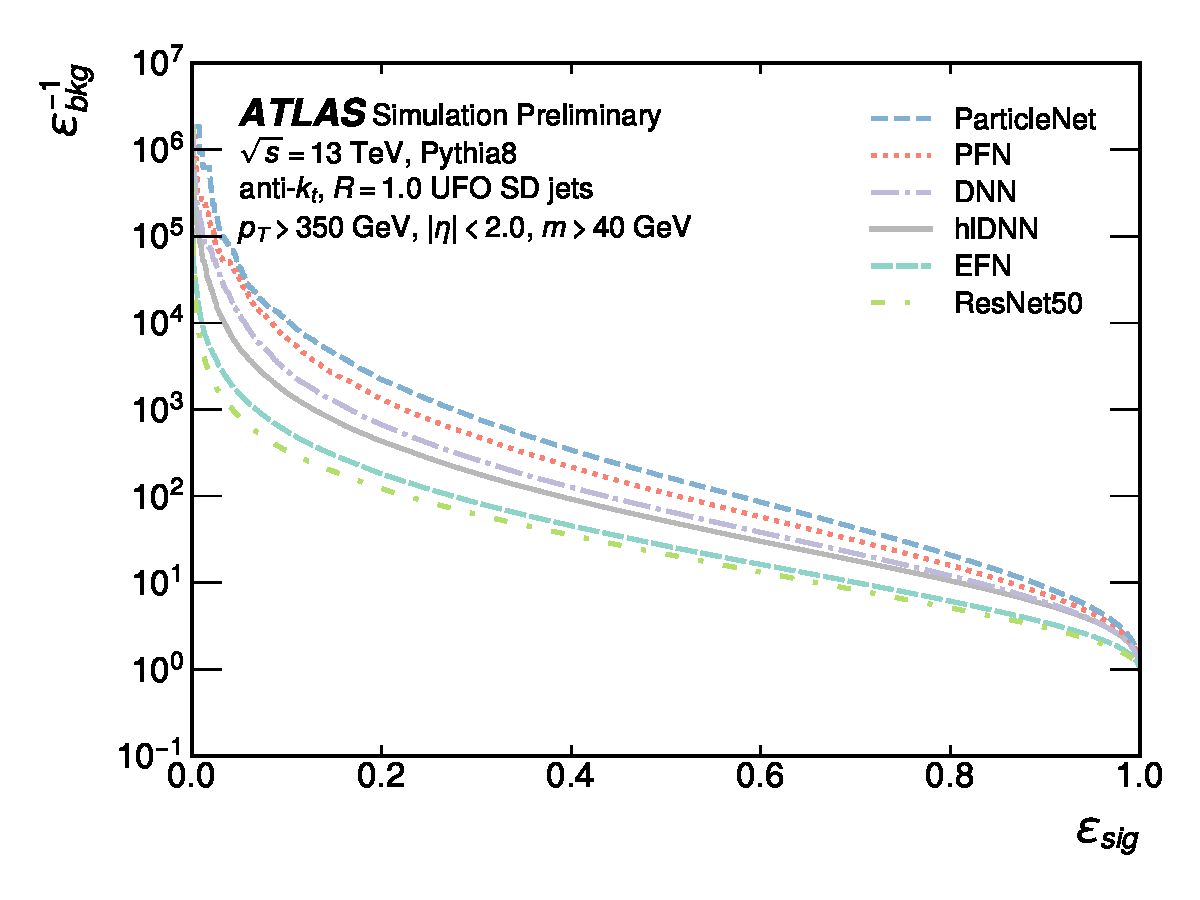
\includegraphics[width=0.75\linewidth]{figures/ch4/roc.pdf}
    \caption{ROC curves for the five top quark taggers evaluated on the full simulation test set. The vertical axis shows the inverse background rejection $\varepsilon^{-1}_\text{bkg}$ and the horizontal axis shows the signal efficiency $\varepsilon_\text{sig}$. All constituent-based taggers outperform the hlDNN expert-feature baseline, with ParticleNet achieving the highest background rejection across all working points.}
    \label{fig:roc}
\end{figure}

\renewcommand{\arraystretch}{1.5}
\begin{table}[]
    \centering
    \caption{The performance of each top quark tagger is measured with several metrics evaluated on the testing set. AUC is the area under the receiving-operator-characteristic curve, ACC is the accuracy, and $\varepsilon^{-1}_{bkg}$ is the inverse background efficiency (or background rejection) evaluated at working points which yield a given signal efficiency ($\varepsilon_{sig}$) across the entire testing set. For all metrics, a higher value means better performance, and the table is sorted by increasing AUC. The uncertainty reported on the metrics is the quadrature sum of the uncertainty from the finite statistics of the testing set and the error from the random initialization of network weights and the stochastic nature of network training.}
    \begin{tabular}{c|c|c|c|c}
        \hline \hline
        Tagger & AUC & ACC & $\varepsilon^{-1}_{bkg}$ @ $\varepsilon_{sig} = 0.5$ & $\varepsilon^{-1}_{bkg}$ @ $\varepsilon_{sig} = 0.8$ \\ \hline
        ResNet 50 & $0.872 \pm 0.006$ & $0.787 \pm 0.006$ & $18.4 \pm 1.1$ & $4.63 \pm 0.2$ \\ 
        EFN & $0.894 \pm 0.001$ & $0.810 \pm 0.001$ & $23.8 \pm 0.5$ & $5.74 \pm 0.07$ \\  
        hlDNN & $0.9374 \pm 0.0001$ & $0.8628 \pm 0.0002$ & $47.2 \pm 0.4$ & $10.36 \pm 0.03$ \\ 
        DNN & $0.9447 \pm 0.0004$ & $0.8715 \pm 0.0008$ & $73.0 \pm 1.3$ & $12.5 \pm 0.1$ \\
        PFN & $0.9502 \pm 0.0004$ & $0.878 \pm 0.001$ & $92.7 \pm 1.8$ & $14.6 \pm 0.2$ \\ 
        ParticleNet & $0.9614 \pm 0.0005$ & $0.895 \pm 0.001$ & $155.8 \pm 3.8$ & $20.6 \pm 0.4$ \\ \hline \hline
    \end{tabular}
    \label{tab:performance_numbers}
\end{table}


ParticleNet is the most performant tagger in the study, outperforming the hlDNN baseline by a factor of roughly 2--3 in background rejection depending on the working point.
This mirrors the result seen in the landscape paper (\Cref{fig:landscape-roc}) and confirms that the performance advantage of constituent-based taggers is not an artifact of fast simulation: it persists under the more challenging conditions of ATLAS full simulation.

The ResNet50 is the worst-performing constituent-based tagger, and notably performs below the hlDNN expert-feature baseline.
This is a significant reversal from the landscape study, where ResNet was among the top performers.
The most likely explanation is the pixelization of the jet image, which imposes a fixed spatial grid on top of the non-uniform calorimeter cell geometry of the ATLAS detector.
The resulting discretization artifacts are severe enough to degrade the network's ability to resolve the substructure patterns that drive its performance.
Delphes fast simulation does not model these non-uniformities, which likely explains why ResNet performed much better in the landscape comparison.

The EFN underperforms the hlDNN despite having access to the full constituent kinematics.
This is a direct consequence of the IRC safety constraint: by weighting constituent features by their $p_T$ fraction before aggregation, the EFN is prevented from utilizing the soft radiation patterns that carry significant discriminating information for top versus QCD classification.
This limitation in raw performance has a counterpart advantage, however, as the EFN's robustness against systematic effects will be discussed in the following section.

Finally, \Cref{fig:br-pt} shows the background rejection as a function of jet $p_T$ at the 50\% and 80\% signal efficiency working points.

\begin{figure}[tb]
    \centering
    \begin{subfigure}[b]{0.48\textwidth}
        \centering
        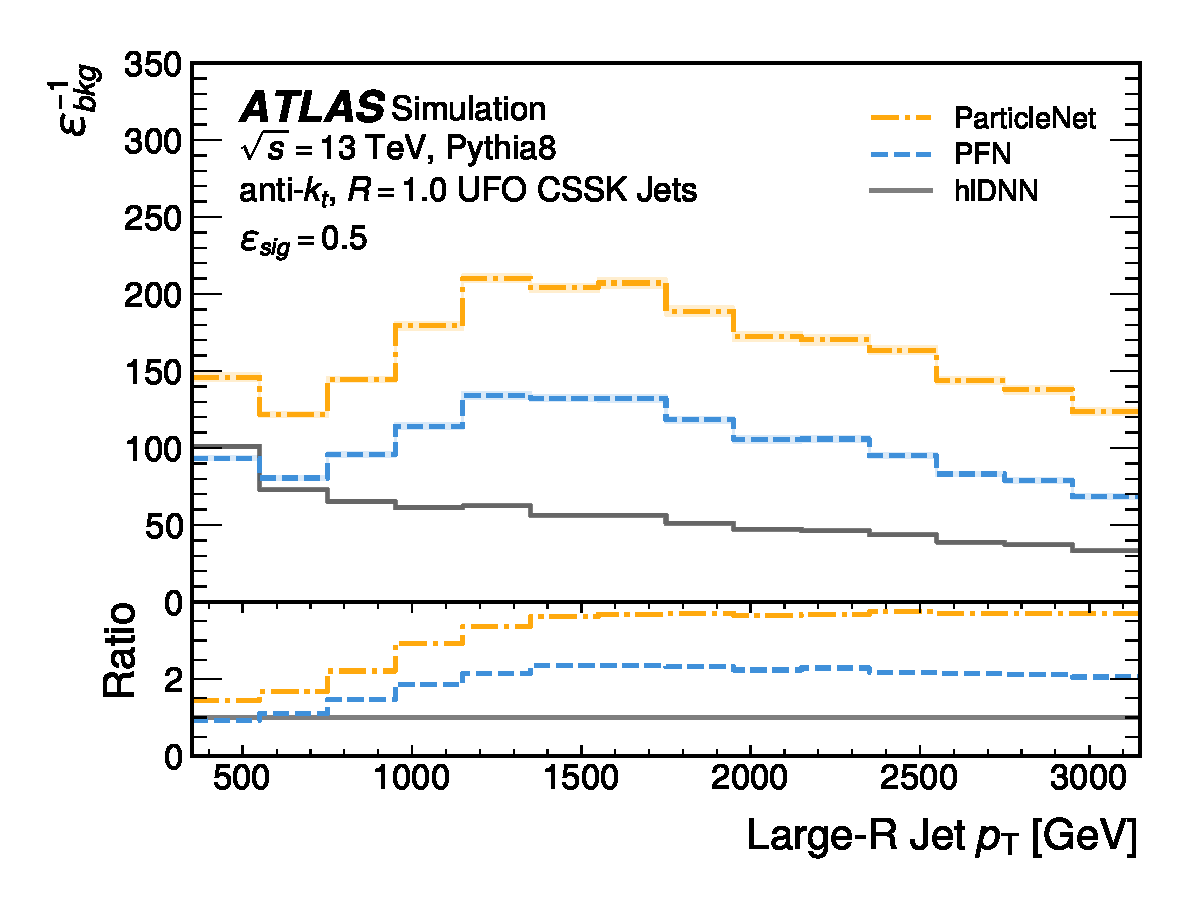
\includegraphics[width=\linewidth]{figures/ch4/br_50.pdf}
        \caption{Background rejection at $\varepsilon_\text{sig} = 50\%$.}
        \label{fig:br-50}
    \end{subfigure}
    \hfill
    \begin{subfigure}[b]{0.48\textwidth}
        \centering
        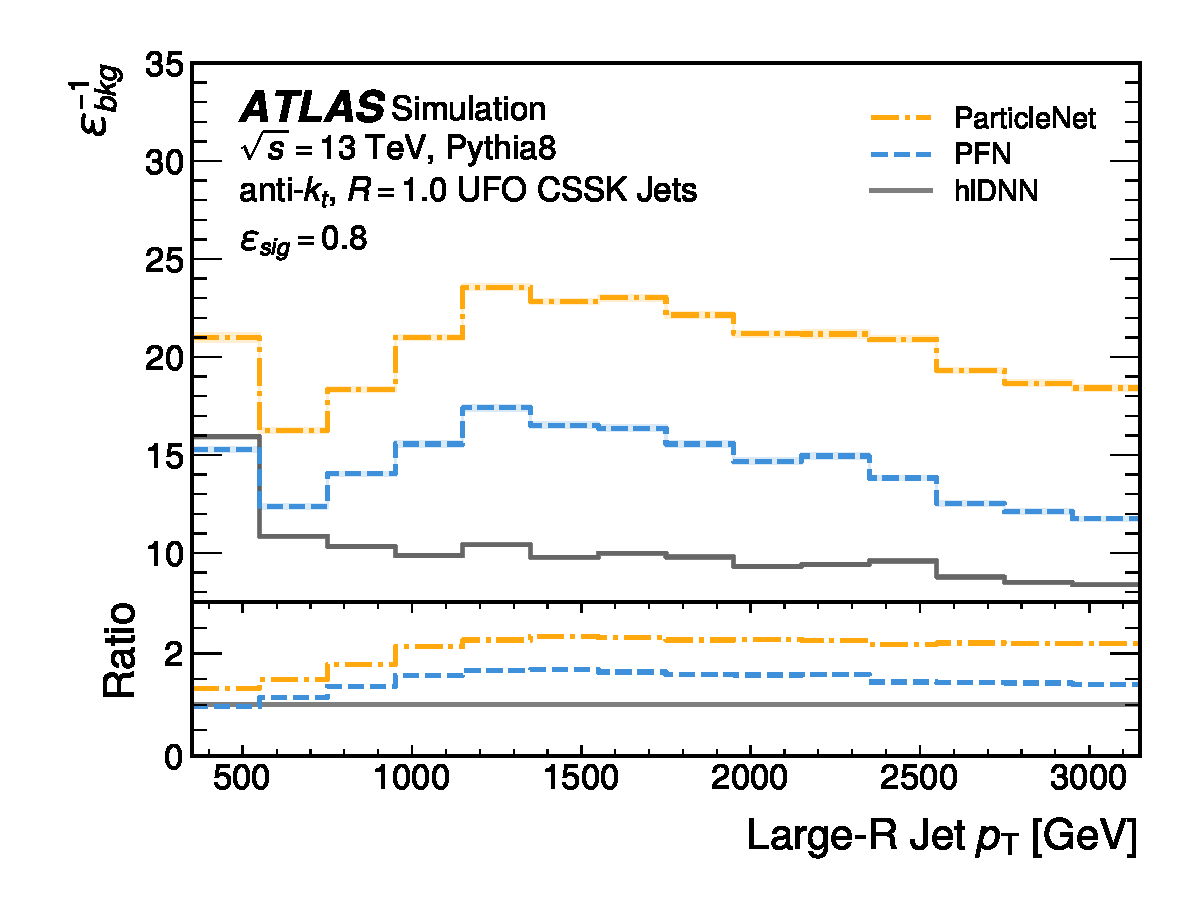
\includegraphics[width=\linewidth]{figures/ch4/br_80.pdf}
        \caption{Background rejection at $\varepsilon_\text{sig} = 80\%$.}
        \label{fig:br-80}
    \end{subfigure}
    \caption{Background rejection as a function of jet $p_T$ at fixed signal efficiency working points of 50\% (left) and 80\% (right). The hlDNN background rejection falls monotonically with increasing $p_T$, consistent with the expectation that the three-pronged substructure of the top decay becomes increasingly difficult to resolve as the jet grows more collimated. Constituent-based taggers show a different behavior, with peak performance in the intermediate $p_T$ range, a trend that is not yet fully understood but may reflect the greater abundance of training statistics at moderate $p_T$.}
    \label{fig:br-pt}
\end{figure}

The hlDNN background rejection falls monotonically with increasing jet $p_T$.
This is physically intuitive: as the top quark becomes more boosted, its three decay products are emitted with smaller angular separations, and the three-pronged substructure becomes increasingly difficult to resolve against the finite angular resolution of the calorimeter.
In the limit of very large $p_T$, all decay products are contained within a single calorimeter cell and the jet images of top and QCD jets become indistinguishable.

The constituent-based taggers display a qualitatively different behavior.
Their background rejection peaks in the intermediate $p_T$ range rather than at low $p_T$, and they degrade more slowly at high $p_T$ than the hlDNN.
The origin of this behavior is not fully understood.
One plausible contributing factor is that the training dataset contains the most jets in the intermediate $p_T$ range (since the flat $p_T$ reweighting has a finite reach), so the networks are better optimized at the $p_T$ values where training statistics are most abundant.
Regardless of origin, the result is that constituent-based taggers maintain a larger performance advantage over the hlDNN baseline precisely in the high-$p_T$ regime where boosted object reconstruction is most relevant for new physics searches.

\section{Systematic Uncertainty Quantification}
\label{sec:systematic-uq}

\section{The Future of Jet Classification}
\label{sec:tagging-future}

